\section{~Compilation and results}
\label{sec:Results}

\input compil_table

A compilation of the various contributions to \amuhadLO and to \dahadZ, as well as the total 
results are given in Table~\ref{tab:results}. The experimental uncertainties are separated
into statistical, channel-specific systematic, and common systematic contributions
that are correlated with at least one other channel. 
\begin{figure*}[t]
  \centering
  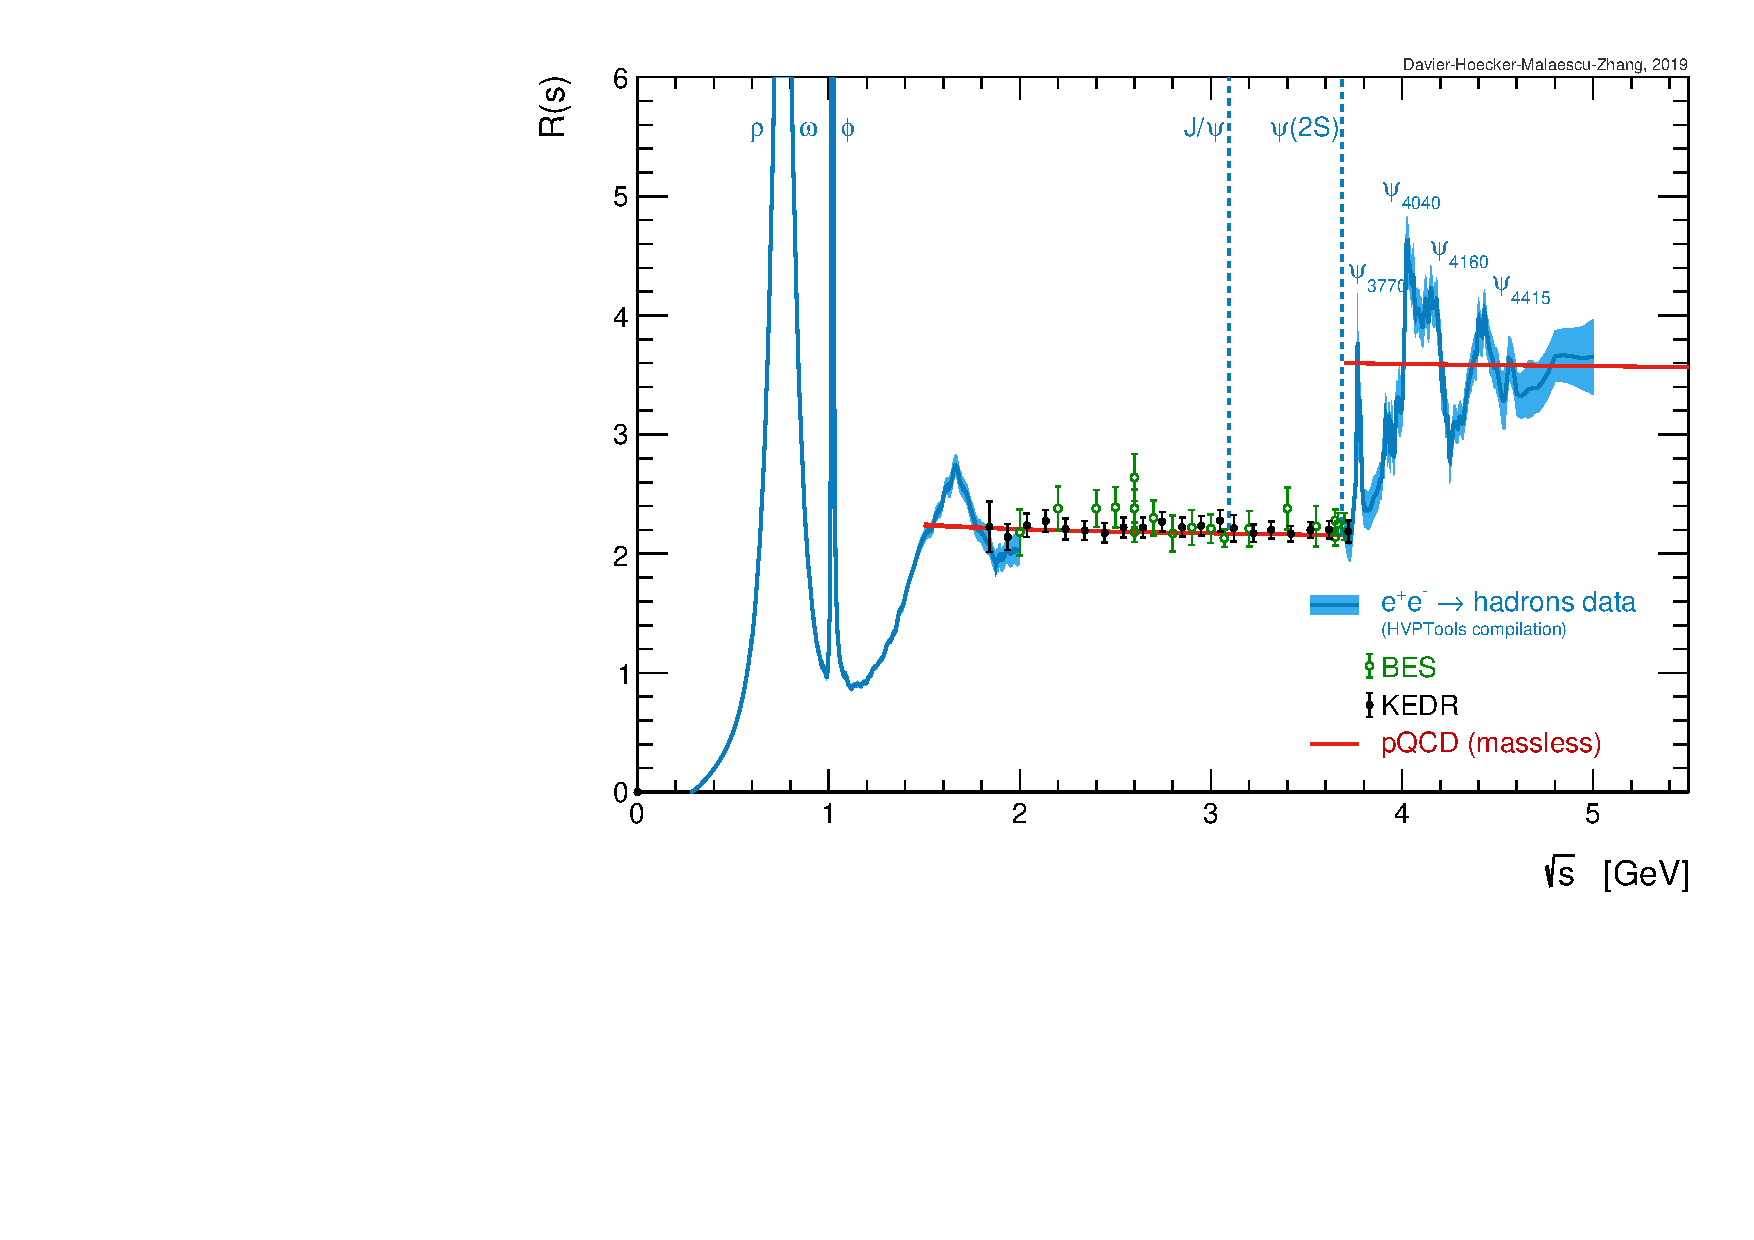
\includegraphics[width=12.5cm]{Figures/R.pdf}
  \vspace{0.2cm}
  \caption{
             The total hadronic \ee annihilation rate $R$ as a function of centre-of-mass energy. Inclusive measurements from BES~\cite{besR}  
             and KEDR~\cite{kedr-r-1,kedr-r-2} are shown as data points,
             while the sum of exclusive channels from this analysis is given by the narrow blue bands. Also shown for the purpose of illustration is the prediction from massless perturbative QCD (solid red line). 
}
  \label{fig:R}
\end{figure*}
The contributions from the $J/\psi$ and $\psi(2S)$ resonances in Table~\ref{tab:results} are obtained by numerically integrating the corresponding undressed\footnote{The undressing uses the BABAR programme {\tt AFKVAC}, correcting for both leptonic  and hadronic VP effects. The hadronic part is obtained from a numerical integration over cross section data for the continuum, supplemented by analytical expressions for the contributions of narrow resonances including both their real and imaginary components. The resulting correction factors reduce the $J/\psi$ and $\psi(2S)$ contributions to \amuhadLO by about 4\% and are known to a precision of better than $10^{-3}$.} Breit-Wigner lineshapes. The uncertainties in the integrals are dominated by the knowledge of the corresponding electronic width $\Gamma_{R\to ee}$ 
for which we use the values $5.53 \pm 0.10\;$keV for $R=J/\psi$ and $2.34 \pm 0.04\;$keV for $R=\psi(2S)$~\cite{pdg}.

Sufficiently far from the quark thresholds we use four-loop~\cite{baikov} perturbative QCD, including ${\cal O}(\as^2)$ quark mass corrections~\cite{kuhnmass}, to compute the inclusive hadronic cross section. Nonperturbative contributions at $1.8\:\gev$ were determined from data~\cite{dh98} and found to be small. The uncertainties of the $R_{\rm QCD}$ contributions given in Table~\ref{tab:results} are obtained from the quadratic sum of the uncertainty in $\as$  (we use $\asZ=0.1193\pm0.0028$ from the fit to  $Z$ precision data~\cite{gfitter}), the truncation of the perturbative series (we use the full four-loop contribution as systematic uncertainty), the  difference between fixed-order perturbation theory  (FOPT) and, so-called, contour-improved perturbation theory (CIPT)~\cite{ledibpich}, as well as quark mass uncertainties (we use the values and uncertainties from Ref.~\cite{pdg}). The former three uncertainties are taken to be fully correlated between the various energy regions (see Table~\ref{tab:results}), whereas the (smaller) quark-mass uncertainties are taken to be uncorrelated. 

To examine the transition region between the sum of exclusive measurements and QCD we have computed \amuhadLO and \dahadZ in the narrow energy interval $1.8$--$2.0\;\gev$. For the former quantity we find $7.65  \pm 0.31$ and $8.30 \pm 0.09$ for data and QCD, respectively. The full difference of $0.65$ ($0.28\cdot10^{-4}$ in the case of \dahadZ) is assigned as additional systematic uncertainty, labelled by ``dual" subscripts in Table~\ref{tab:results}. It accounts for possible low-mass quark-hadron duality violation effects in the perturbative QCD approximation that we use for this interval to avoid systematic effects due to  unmeasured high-multiplicity channels. 

Figure~\ref{fig:R} shows the total hadronic \ee annihilation rate $R$ versus centre-of-mass energy as obtained from the sum of exclusive data below 2$\;$GeV and from inclusive data between 1.8 and 5$\;$GeV.\footnote{We have verified that the integration of the finely binned $R$ distribution shown in Fig.~\ref{fig:R}, together with its covariance matrix, accurately reproduces the \amuhadLO and \dahadZ results obtained by summing the exclusive modes below 1.8$\;$GeV  in Table~\ref{tab:results}.} Also indicated are the perturbative QCD prediction above 1.5$\;$GeV and the analytical narrow $J/\psi$ and $\psi(2S)$ resonances.

\vspace{0.0cm}
\paragraph*{\bf\em Muon magnetic anomaly\\[0.2cm] } 

Adding all lowest-order hadronic contributions together gives
\beq
\label{eq:amuhadlo}
   \amuhadLO = 694.0 \pm 4.0\,,
\eeq
which is dominated by experimental systematic uncertainties (\cf Table~\ref{tab:results} for a separation of the total uncertainty into its components), with an uncertainty of 2.8 originating from the BABAR versus KLOE discrepancy in the \pp channel. The new result is $0.9$ units larger than  our previous evaluation~\cite{dhmz2017}, $693.1\pm3.4$, mostly because we symmetrised the new BABAR/KLOE systematic uncertainty. The total uncertainty is increased by 18\%.  The result without the additional BABAR/KLOE systematic uncertainty is $693.1\pm3.2$.

Adding to~(\ref{eq:amuhadlo}) the contributions from higher order hadronic loops, $-9.87 \pm 0.09$ (NLO) and $1.24\pm0.01$ (NNLO)~\cite{amu-hadnlo}, hadronic light-by-light scattering, $10.5\pm 2.6$~\cite{amu-lbl},  as well as QED, $11\,658\,471.895 \pm 0.008$~\cite{amu-qed} (see also~\cite{pdgg-2rev} and references therein), and electroweak effects, $15.36 \pm 0.10$~\cite{amu-ew},\footnote{When adjusting~\cite{wjm}  the new full 2-loop calculation in Ref.~\cite{amu-ew-num} to physical quark masses, it reproduces the value obtained in~\cite{amu-ew}.} we obtain the complete SM prediction
\beq
\label{eq:amusm}
  \amuSM = 11\,659\,183.1 \pm 4.0 \pm 2.6 \pm 0.1~(4.8_{\rm tot})\,,
\eeq
where the uncertainties account for lowest and higher order hadronic, and 
other contributions, respectively. The result~(\ref{eq:amusm}) deviates from the 
experimental value, $\amuExp=11\,659\,209.1 \pm 5.4 \pm 3.3$~\cite{bnl,pdgg-2rev}, 
by $26.0 \pm 7.9$ ($3.3\sigma$).

A compilation of recent SM predictions for \amu compared with the experimental
result is given in Fig.~\ref{fig:amures}.

\vspace{0.0cm}
\paragraph*{\bf\em Running electromagnetic coupling at \boldmath$m_Z^2$ \\[0.2cm]}

The sum of all quark-flavour terms from Table~\ref{tab:results} gives for the 
hadronic contribution to the running of \aZ
\beq
\label{eq:dahad}
   \dahadZ   = (275.3 \pm 1.0)\cdot 10^{-4}\,,
\eeq
the uncertainty of which is dominated by data systematic effects ($0.7\cdot 10^{-4}$) and the uncertainty in the QCD prediction ($0.6\cdot 10^{-4}$). The use of the same inputs with different integration kernels in the calculations induces a correlation of $+44$\% between the $a_\mu^\mathrm{had, LO}$ and $\Delta \alpha_\mathrm{had}(m^2_Z)$ uncertainties. The result without the new BABAR/KLOE systematic uncertainty is $275.2\pm0.9$.

Adding to~(\ref{eq:dahad}) the four-loop leptonic contribution, $\Delta\alpha_{\rm lep} (m_Z^2)=(314.979 \pm 0.002)\cdot 10^{-4}$~\cite{sturm}, 
one finds
\beq
   \alpha^{-1}(m_Z^2) = 128.947 \pm 0.013\,.
\eeq
The current uncertainty on $ \alpha(m_Z^2)$ is sub-dominant in the SM prediction of the $W$-boson mass (the dominant uncertainties are due to the top mass and of theoretical origin), but dominates the prediction of $\sin^2\theta_{\rm eff}^\ell$, which, however, is about twice more accurate than the combination of all present measurements~\cite{gfitter}.

\begin{figure}[t]
\vspace{0.1cm}

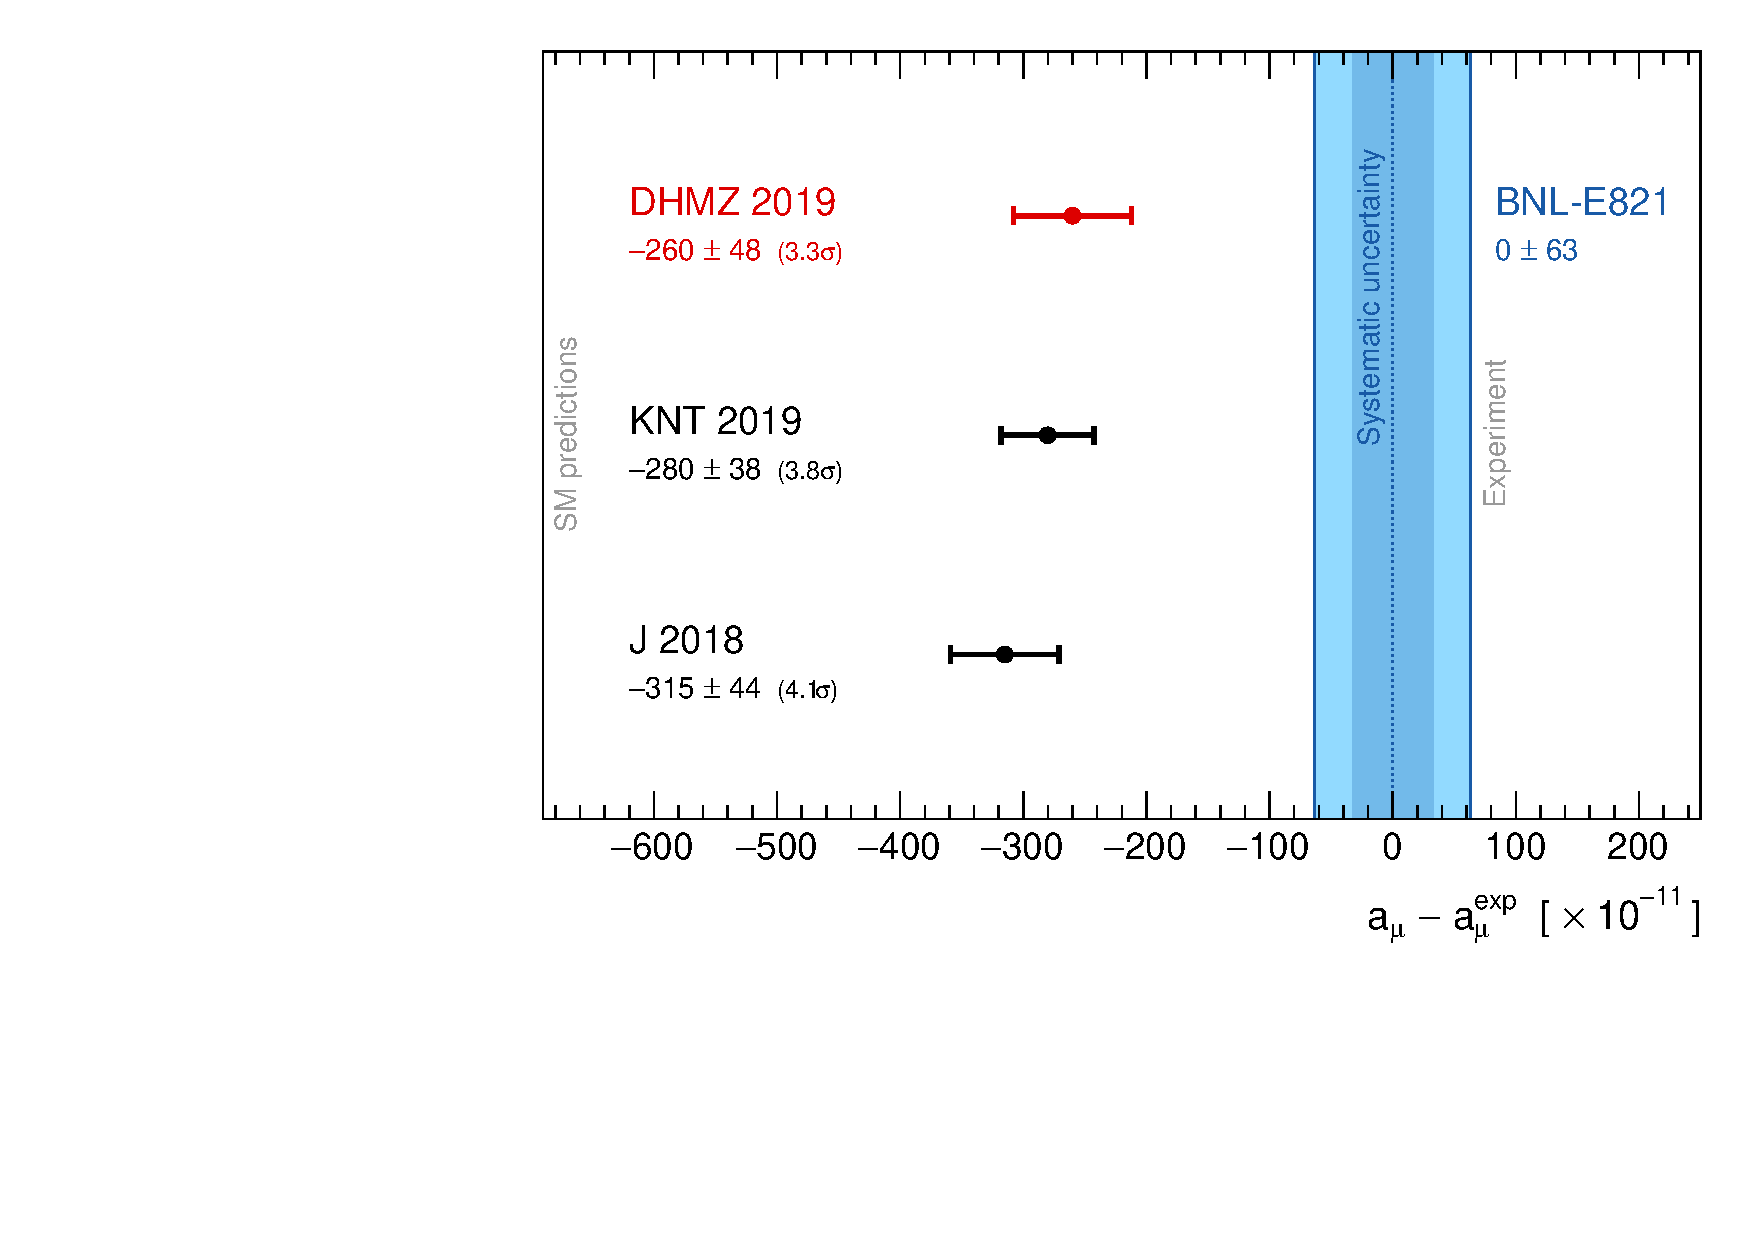
\includegraphics[width=\columnwidth]{Figures/amures.pdf}
\vspace{-0.3cm}
\caption{ 
        Compilation of recent data-driven results for $\amuSM$ (in units of $10^{-10}$), subtracted by the central value of the experimental average~\cite{bnl,pdgg-2rev}.  The blue vertical band indicates the experimental uncertainty, with the darker inlet representing the experimental systematic uncertainty. The representative SM predictions are taken from KNT 2019~\cite{knt19}, J 2018~\cite{jeger},  and this work (DHMZ 2019). }
\label{fig:amures}
\end{figure}

\section{~Conclusions and perspectives}

Using newest available $e^+e^-\to {\rm hadrons}$ cross-section data we have reevaluated the lowest-order hadronic vacuum polarisation contribution to the Standard Model prediction of the anomalous magnetic moment of the muon, and the hadronic contribution to the running electromagnetic coupling strength at the $Z$-boson mass. For the former quantity we find $\amuhadLO = (694.0 \pm 4.0)\cdot 10^{-10}$. In spite of new data and the use of a more precise fit to evaluate the threshold region up to 0.6$\;$GeV, the uncertainty on this contribution has increased to 0.6\% since our last evaluation~\cite{dhmz2017}, due to the addition of a new systematic uncertainty to account for a global discrepancy between \pp data from BABAR and KLOE.
Resolving this discrepancy would allow to reduce the \amuhadLO uncertainty by 20\%.\footnote{The contribution of the $\pp$ channel to the total \amuhadLO uncertainty-squared is $71\%$.} 

\sloppy
The discrepancy between measurement and complete Standard Model prediction remains at a non-conclusive $3.3\sigma$ level. The new Fermilab $g-2$ experiment currently in operation~\cite{fnal-g-2} aims at up to four times better ultimate precision and has the potential to clarify the situation. 

To match the precision of the new experiment  further progress is  needed to reduce the uncertainty on \amuhadLO from dispersion relations. New analyses of the dominant $\pip\pim$ channel are underway at the BABAR, CMD-3 and SND experiments for which a systematic uncertainty below 0.5\% may be reachable.  It is also important to  improve the precision of the $\pip\pim\piz$ and $K^+ K^-$ channels. The new Belle-2 experiment at the KEK Super-B factory will also contribute to measuring hadronic cross sections via the ISR method once the detector performance is fully understood and sufficient statistics has been accumulated. 

Independently of the data-driven approach, lattice QCD calculations of \amuhadLO  are  also progressing albeit not yet reaching competitive  precision~\cite{Lattice-amu}.

The determination of \amuhadLO is closing in on the estimated  uncertainty of the hadronic light-by-light scattering contribution \amuhadLBL of  $2.6\cdot10^{-10}$, which appears irreducible at present. Here only phenomenological models have been used so far and lattice QCD calculations could have a strong impact~\cite{Lattice-lbl}, as well as a new promising dispersive approach~\cite{Hoferichter:2018kwz}. 
